\documentclass[aspectratio=169]{beamer}

\mode<presentation>
{
  \setbeamertemplate{background canvas}[square]
  \pgfdeclareimage[width=6em,interpolate=true]{dsailogo}{../dsai-logo}
  \pgfdeclareimage[width=6em,interpolate=true]{erasmuslogo}{../erasmus-logo}
  \titlegraphic{\pgfuseimage{dsailogo} \hspace{0.2in} \pgfuseimage{erasmuslogo}}
  %\usetheme{default}
  \usetheme{Madrid}
  \usecolortheme{rose}
  \usefonttheme[onlysmall]{structurebold}
}

\usepackage{pgf,pgfarrows,pgfnodes,pgfautomata,pgfheaps,pgfshade}
\usepackage{amsmath,amssymb}
\usepackage{graphics}
\usepackage{ragged2e}
\usepackage[latin1]{inputenc}
\usepackage{colortbl}
\usepackage[absolute,overlay]{textpos}
\setlength{\TPHorizModule}{30mm}
\setlength{\TPVertModule}{\TPHorizModule}
\textblockorigin{10mm}{10mm}
\usepackage[english]{babel}
\setbeamercovered{dynamic}

\AtBeginSection[]{
  \begin{frame}<beamer>
  \frametitle{Outline}
  \tableofcontents[currentsection]
  \end{frame}
}

\title[Computer Vision]{Computer Vision\\Estimation}
\author{dsai.asia}
\institute[]{Asia Data Science and Artificial Intelligence Master's Program}
\date{}

% My math definitions

\renewcommand{\vec}[1]{\boldsymbol{#1}}
\newcommand{\mat}[1]{\mathtt{#1}}
\newcommand{\ten}[1]{\mathcal{#1}}
\renewcommand{\null}[1]{{\cal N}(#1)}
\def\Rset{\mathbb{R}}
\def\Pset{\mathbb{P}}
\DeclareMathOperator*{\argmax}{argmax}
\DeclareMathOperator*{\argmin}{argmin}
\def\norm{\mbox{$\cal{N}$}}

\newcommand{\stereotype}[1]{\guillemotleft{{#1}}\guillemotright}

\newcommand{\myfig}[3]{\centerline{\includegraphics[width={#1}]{{#2}}}
    \centerline{\scriptsize #3}}

\begin{document}

%%%%%%%%%%%%%%%%%%%%%%%%%%%%%%%%%%%%%%%%%%%%%%%%%%%%%%%%%%%%
%%             CONTENTS START HERE

%\setbeamertemplate{navigation symbols}{}

\frame{\titlepage}

%--------------------------------------------------------------------
%\part<presentation>{Part name}
%
%\frame{\partpage}

\begin{frame}
\frametitle{Readings}

Readings for these lecture notes:
\begin{itemize}
\item[-] Hartley, R., and Zisserman, A. {\em Multiple View Geometry in
    Computer Vision}, Cambridge University Press, 2004, Chapter 4.
\item[-] Tomasi, C. {\em Mathematical Modeling of Continuous Systems},
    online lecture notes from Duke University, 2004.
\end{itemize}

\medskip

If you are unfamiliar with the mathematics used in these lecture
notes, study Carlo Tomasi's beautiful lecture notes.  You'll find the
notes on the course Web site under ``Readings.''

\medskip

These notes contain material $\copyright$ Hartley and Zisserman
(2004) and Tomasi (2004).

\end{frame}

%--------------------------------------------------------------------
\section{Introduction}
%--------------------------------------------------------------------

\begin{frame}
\frametitle{Introduction}
\framesubtitle{Estimation Problems}

In vision, we are frequently confronted with \alert{estimation} problems
in which parameters of some function must be estimated from measurements.

\medskip

Some examples of important estimation problems:

\begin{itemize}
\item \alert{2D homography}: Given a set of points $\vec{x}_i$ in
  $\Pset^2$ and corresponding points $\vec{x}_i'$ in $\Pset^2$,
  find a homography taking each $\vec{x}_i$ to $\vec{x}_i'$.
\item \alert{3D to 2D camera projection}: Given a set of points
  $\vec{X}_i$ in 3D space and corresponding points $\vec{x}_i$
  in an image, find the 3D to 2D projective mapping taking each
  $\vec{X}_i$ to $\vec{x}_i$.
\item \alert{Fundamental matrix computation}: Given a set of
  points $\vec{x}_i$ in one image and a set of corresponding
  points $\vec{x}_i'$ in another image, find the fundamental
  matrix $\mat{F}$ relating the two images.
\item \alert{Trifocal tensor computation}: Given a set of
  point correspondences $\vec{x}_i \leftrightarrow \vec{x}_i'
  \leftrightarrow \vec{x}_i''$ across three images, compute the
  trifocal tensor $\ten{T}_i^{jk}$ relating points or lines in
  three views.
\end{itemize}

\end{frame}

\begin{frame}
\frametitle{Introduction}
\framesubtitle{Homography estimation}

First we'll consider homography estimation.

\medskip

We have a set of points $\vec{x}_i$ and corresponding points
$\vec{x}_i'$.  We want to compute $\mat{H}$ such that $\forall i,
\mat{H} \vec{x}_i = \vec{x}_i'$.

\medskip

How many points do we need?
\begin{itemize}
\item We already saw that each point
correspondence gives us 2 constraints (equations), one for the $x$
component and one for the $y$ component.
\item Since $\mat{H}$ has 8
degrees of freedom we need at least 4 correspondences.
\end{itemize}

\end{frame}

\begin{frame}
\frametitle{Introduction}
\framesubtitle{Cost functions}

We know that 4 correspondences yields an \alert{exact solution}.

\medskip

Due to \alert{measurement error} and \alert{correspondence error} we
should get \alert{more than 4 correspondences} then find the
homography $\mat{H}$ minimizing some \alert{cost function}.

\medskip

\begin{block}{Gold Standard algorithm (Hartley and Zisserman, 2004)}
An estimation algorithm minimizing the cost function that
is \alert{the best possible cost function} under certain assumptions.
\end{block}

\medskip

All algorithms should be evaluated with respect to the Gold Standard.

\end{frame}

%--------------------------------------------------------------------
\section{Direct Linear Transform (DLT)}
%--------------------------------------------------------------------

\begin{frame}
\frametitle{Direct Linear Transform (DLT)}
\framesubtitle{Another view of the homography estimation problem}

Now we'll look at another way to derive the exact linear estimate of
$\mat{H}$ from 4 points.

\medskip

For corresponding points $\vec{x}_i \leftrightarrow \vec{x}_i'$ we
want $\vec{x}_i' = k_i \mat{H} \vec{x}_i$ for some nonzero scaling
factor $k$.

\medskip

Thus we can say that $\vec{x}_i'$ and $\mat{H}\vec{x}_i$ must be collinear.

\medskip

Recall that the \alert{cross product} of two collinear vectors is the
0 vector.

\medskip

This means we can write this constraint in the form
$\vec{x}_i' \times \mat{H} \vec{x}_i = \vec{0}$.

\end{frame}

\begin{frame}
\frametitle{Direct Linear Transform (DLT)}
\framesubtitle{Deriving the linear system}

Let's use $\vec{h}^{j}$ to denote the $j$-th row of $\mat{H}$ written
as a vector.  Then we have
\begin{equation*}
\mat{H}\vec{x}_i = \begin{pmatrix} \vec{h}^{1T}\vec{x}_i \\
\vec{h}^{2T}\vec{x}_i \\ \vec{h}^{3T}\vec{x}_i \end{pmatrix}.
\end{equation*}

\medskip

Now if $\vec{x}_i' = (x_i',y_i',w_i')^T$, the cross product can be written
\begin{equation*}
\vec{x}_i' \times \mat{H} \vec{x}_i = \begin{pmatrix}
y_i' \vec{h}^{3T}\vec{x}_i - w_i' \vec{h}^{2T}\vec{x}_i \\
w_i' \vec{h}^{1T}\vec{x}_i - x_i' \vec{h}^{3T}\vec{x}_i \\
x_i' \vec{h}^{2T}\vec{x}_i - y_i' \vec{h}^{1T}\vec{x}_i \end{pmatrix}.
\end{equation*}

\end{frame}

\begin{frame}
\frametitle{Direct Linear Transform (DLT)}
\framesubtitle{Deriving the linear system}

Since we want the cross product to be the zero vector, we can write
the linear system
\begin{equation*}
\begin{bmatrix}
\vec{0}^T        & -w_i'\vec{x}_i^T & y_i'\vec{x}_i^T  \\
w_i'\vec{x}_i^T  & \vec{0}^T        & -x_i'\vec{x}_i^T \\
-y_i'\vec{x}_i^T & x_i'\vec{x}_i^T  & \vec{0}^T        \end{bmatrix} 
\begin{pmatrix} \vec{h}^1 \\ \vec{h}^2 \\ \vec{h}^3 \end{pmatrix} =
\vec{0}.
\end{equation*}

\medskip

We have three linear equations in 9 unknowns.
The third equation is actually a linear combination of the first
two.\footnote{To convince yourself of this, use the factor $-x_i'/w_i'$
for the first equation and $-y_i'/w_i'$ for the second equation.}
So we can drop it (see next slide)...

\end{frame}

\begin{frame}
\frametitle{Direct Linear Transform (DLT)}
\framesubtitle{Deriving the linear system}

Dropping the redundant third equation in the parameters of $\mat{H}$, we have:
\begin{equation}
\label{dlt-eqn}
\mat{A}_i\vec{h} = 
\begin{bmatrix}
\vec{0}^T        & -w_i'\vec{x}_i^T & y_i'\vec{x}_i^T  \\
w_i'\vec{x}_i^T  & \vec{0}^T        & -x_i'\vec{x}_i^T \end{bmatrix}
\begin{pmatrix} \vec{h}^1 \\ \vec{h}^2 \\ \vec{h}^3 \end{pmatrix} =
\vec{0}.
\end{equation}
However, if $w_i' = 0$ we have an ideal point, and the first two
equations become linearly dependent.  In this case we should use the
third equation and the first or second equation, or just use all three
equations all the time.

\end{frame}

\begin{frame}
\frametitle{Direct Linear Transform (DLT)}
\framesubtitle{Deriving the linear system}

With 8 equations in 9 unknowns, $\mat{A}$ is $8\times 9$ and has rank
8.  It has a one-dimensional null space and we obtain $\vec{h} =
\null{\mat{A}}$.

\medskip

If we have \alert{more than 4 correspondences} the system
$\mat{A}\vec{h}=\vec{0}$ will be \alert{over-determined}:
\begin{itemize}
\item With \alert{perfect measurement}, the rank of $\mat{A}$ would
  still be 8 and it would still have a one-dimensional null space.
\item But \alert{measurement noise} means no exact solution.
\item So we try to find the vector $\vec{h}$ minimizing some \alert{cost
  function}.
\end{itemize}

\medskip

Since we want $\mat{A}\vec{h}$ to be as close as possible to
$\vec{0}$, a sensible cost function is the \alert{norm} of
$\mat{A}\vec{h}$, i.e., $\|\mat{A}\vec{h}\|$.

\medskip

However we must avoid the \alert{trivial solution} $\vec{h}=\vec{0}$,
so we impose a constraint $\|\vec{h}\|=1$.  This is OK since $\mat{H}$
is homogeneous.

\end{frame}

\begin{frame}
\frametitle{Direct Linear Transform (DLT)}
\framesubtitle{Solving the linear system}

So now we have the minimization problem
\begin{equation*}
\hat{\vec{h}} = \argmin_{\vec{h}} \|\mat{A}\vec{h}\|, \text{subject to }
\|\vec{h}\|=1.
\end{equation*}
whose solution is to let $\vec{h}$ be the unit eigenvector of
$\mat{A}^T\mat{A}$ with the smallest eigenvalue, or the unit singular
vector of $\mat{A}$ corresponding to the smallest singular value of
$\mat{A}$.

\medskip

\alert{This is important to remember:} to solve an overconstrained
homogeneous linear system $\mat{A}\vec{x}=\vec{0}$ by minimizing
$\|\mat{A}\vec{h}\|$ subject to $\|\vec{h}\|=1$, we \alert{perform SVD
  on $\mat{A}$} (see next section) or \alert{compute the eigenvector
  corresponding to the smallest eigenvalue of $\mat{A}^T\mat{A}$}.

\end{frame}

\begin{frame}
\frametitle{Direct Linear Transform (DLT)}
\framesubtitle{The basic DLT for $\mat{H}$}

\begin{block}{DLT: Objective}
Given $n \ge 4$ 2D to 2D point correspondences $\{ \vec{x}_i
\leftrightarrow \vec{x}_i' \}$, determine the 2D homography matrix
$\mat{H}$ such that $\vec{x}_i' = \mat{H}\vec{x}_i$.
\end{block}

\begin{block}{DLT: Algorithm}
\begin{itemize}
\item[(i)] For each correspondence $\vec{x}_i \leftrightarrow
  \vec{x}_i'$, compute the matrix $\mat{A}_i$ as in equation
  (1).  When $w_i'=0$, use different rows.
\item[(ii)] Assemble the $n$ $2\times 9$ matrices $\mat{A}_i$ into a
  single $2n\times 9$ matrix $\mat{A}$.
\item[(iii)] Obtain the SVD $\mat{A}=\mat{U}\mat{D}\mat{V}^T$.  The
  unit singular vector (column of $\mat{V}$) corresponding to the
  smallest singular value (diagonal element of $\mat{D}$) is the
  desired $\vec{h}$.
\item[(iv)] Rearrange $\vec{h}$ to obtain $\mat{H}$.
\end{itemize}
\end{block}

\end{frame}

\begin{frame}
\frametitle{Direct Linear Transform (DLT)}
\framesubtitle{Similar approaches}

Other methods: we can select one element of $\vec{h}$ to be equal to 1
(or any other arbitrary value) to obtain an inhomogeneous linear
system which can be solved by the usual least squares methods (see
text).

\medskip

We can also compute $\mat{H}$ in the same way using line
correspondences or conic correspondences.  The derivations are quite
similar.

\end{frame}

\begin{frame}
\frametitle{Direct Linear Transform (DLT)}
\framesubtitle{Example code}

For example code for the DLT in Octave, see \texttt{dlt\_demo.m} on
the course Web site.

\end{frame}

%--------------------------------------------------------------------
\section{Singuar value decomposition (SVD)}
%--------------------------------------------------------------------

\begin{frame}
\frametitle{Singular value decomposition (SVD)}
\framesubtitle{Definition}

The SVD is an incredibly useful factorization, particularly for the
kinds of estimation problems that come up in computer vision.

\medskip

\begin{block}{Singular Value Decomposition}
Given an $m\times n$ matrix $\mat{A}$, the \alert{singular value
  decomposition} of $\mat{A}$ is
\begin{equation*}
\mat{A} = \mat{U}\mat{D}\mat{V}^T
\end{equation*}
where the columns of $\mat{U} \in \Rset^{m\times m}$ and $\mat{V} \in
\Rset^{n\times n}$ are orthogonal unit vectors and $\mat{D} \in
\Rset^{m\times n}$ is a diagonal matrix whose elements $\sigma_i$,
with $\sigma_1 \ge \cdots \ge \sigma_p \ge 0$, ($p=\min(m,n)$), are
called the \alert{singular values} of $\mat{A}$.
\end{block}

\end{frame}

\begin{frame}
\frametitle{Singular value decomposition (SVD)}
\framesubtitle{Geometric interpretation}

Writing $\mat{A}=\mat{U}\mat{D}\mat{V}^T$ models the transformation
$\vec{y}=\mat{A}\vec{x}$ as a rotation, a ``stretch'' of the unit
hypershpere into a hyperellipse, and a rotation of the hyperellipse.
Example:

\begin{columns}
\column{1.1in}
\begin{equation*}
\mat{A} = \frac{1}{\sqrt{2}}
\begin{bmatrix}
\sqrt{3} & \sqrt{3} \\
-3 & 3 \\
1 & 1
\end{bmatrix}
\end{equation*}

\column{2.6in}
\myfig{2.5in}{Tomasi-fig3-2}{}

\end{columns}

\vspace{-0.25in}

\centerline{\scriptsize Example from Tomasi (2004), Section 3.}

\end{frame}

\begin{frame}
\frametitle{Singular value decomposition (SVD)}
\framesubtitle{Properties of the SVD}

The SVD has many useful properties:
\begin{itemize}
\item If $m=n$ and $\sigma_i \not= 0, \forall i$, then $\mat{A}$ is
  \alert{invertible}.  The ratio $C=\sigma_1/\sigma_n$ is called the
  \alert{condition number} of $\mat{A}$ and tells us how close
  $\mat{A}$ is to singularity.  When $1/C$ is close to numerical
  precision, we say $\mat{A}$ is \alert{ill-conditioned} and should be
  considered singular.
\item The number of nonzero $\sigma_i$ is the \alert{rank} of
  $\mat{A}$.  Numerically, we must specify a tolerance, e.g.\
  $\epsilon=10^{-6}$, and say the number of singular values greater
  than $\epsilon$ is the rank of $\mat{A}$.
\item We can get the \alert{inverse} or \alert{pseudoinverse} of
  $\mat{A}$ using the SVD: $\mat{A}^{-1}=\mat{V}\mat{D}^{-1}\mat{U}^T$
  or $\mat{A}^+ = \mat{V}\mat{D}_0^{-1}\mat{U}^T$, where
  $\mat{D}_0^{-1}$ is $\mat{D}^{-1}$ for the nonzero singular values
  and 0 otherwise.
\end{itemize}

\end{frame}

\begin{frame}
\frametitle{Singular value decomposition (SVD)}
\framesubtitle{Properties of the SVD}

More properties:
\begin{itemize}
\item The \alert{columns} of $\mat{U}$ corresponding to the
  \alert{nonzero} $\sigma_i$ span the \alert{range} of $\mat{A}$.  The
  columns of $\mat{V}$ corresponding to the zero singular values span
  the null space of $\mat{A}$.
\item The \alert{squares of the nonzero singular values} of $\mat{A}$
  are the \alert{nonzero eigenvalues} of $\mat{A}^T\mat{A}$ and
  $\mat{A}\mat{A}^T$.  The \alert{columns} of $\mat{U}$ are the
  \alert{eigenvectors} of $\mat{A}\mat{A}^T$ and the \alert{columns}
  of $\mat{V}$ are the \alert{eigenvectors} of $\mat{A}^T\mat{A}$.
  Additionally, we can write $\mat{A}\vec{u}_k = \sigma_k \vec{v}_k$
  and $\mat{A}^T\vec{v}_k=\sigma_k\vec{u}_k$ where $\vec{v}_k$ is the
  $k$th column of $\mat{V}$ and $\vec{u}_k$ is the $k$th column of
  $\mat{U}$.
\item The singular values of $\mat{A}$ are related to the
  \alert{Frobenius norm} of $\mat{A}$:
\begin{equation*}
\|\mat{A}\|^2_F = \sum_{i,j}a_{i,j}^2 = \sum_i\sigma_i^2.
\end{equation*}
\end{itemize}

\end{frame}

\begin{frame}
\frametitle{Singular value decomposition (SVD)}
\framesubtitle{Applications}

Here are some of the SVD's many uses:
\begin{itemize}
\item In \alert{inhomogeneous} linear least squares problems
  ($\mat{A}\vec{x}=\vec{b}$), we use the SVD to obtain the
  pseudoinverse of A and let $\vec{x}=\mat{A}^+\vec{b}$.
\item In \alert{homogeneous} least squares problems, when we want to minimize
  $\|\mat{A}\vec{x}\|$ subject to $\|\vec{x}\|=1$, we obtain the SVD
  and let $\vec{x}$ be the last column of $\mat{V}$ (since it is also
  the least eigenvector of $\mat{A}^T\mat{A}$).
\item In some cases we can use the SVD to \alert{enforce constraints
    on an estimated matrix}.  For example, if we obtain an estimate
  $\mat{R}$ of a rotation matrix that is not quite orthogonal, we can
  compute the orthogonal matrix
  $\hat{\mat{R}}=\mat{U}\mat{I}\mat{V}^T$ that is closest to $\mat{R}$
  measured by the Frobenius norm.  We can use a similar approach for
  rank constraints.
\end{itemize}

\end{frame}

%--------------------------------------------------------------------
\section{Cost functions}
%--------------------------------------------------------------------

\begin{frame}
\frametitle{Cost functions}
\framesubtitle{Algebraic distance}

DLT minimizes $\|\mat{A}\vec{h}\|$.  The vector $\vec{\epsilon} =
\mat{A}\vec{h}$ is called the \alert{residual vector}.  Each of the
components of $\vec{\epsilon}$ comes from one of the individual
correspondences generating a row of $\mat{A}$.

\medskip

The part of the vector $\vec{\epsilon}_i$ contributed by one
correspondence $\vec{x}_i \leftrightarrow \vec{x}_i'$ is called the
\alert{algebraic error} for correspondence $i$ and homography
$\mat{H}$.  The norm of $\vec{\epsilon}_i$ is called the
\alert{algebraic distance} between $\vec{x}_i'$ and
$\mat{H}\vec{x}_i$.

\medskip

The algebraic distance is a convenient cost function because it leads
to a straightforward linear solution, but \alert{it is not
geometrically or statistically meaningful}!

\medskip

We will find that \alert{normalization} is crucial to obtaining good
results from algorithms minimizing algebraic error.

\medskip

We will also look at algorithms that use DLT and similar linear
algebraic error-minimizing routines to obtain an initial solution,
then minimize a statistical or geometrical cost function from there.

\end{frame}

\begin{frame}
\frametitle{Cost functions}
\framesubtitle{Geometric error}

Here we'll use $\vec{x}$ to represent a \alert{measured} image point,
$\hat{\vec{x}}$ to denote an \alert{estimated} point, and
$\bar{\vec{x}}$ to represent the \alert{true value} of a point.

\medskip

As a starting point, imagine we have perfect measurements in the first
image and error in the second image.

\medskip

Let $d(\vec{x},\vec{y})$ be the \alert{Euclidean} distance between the
\alert{inhomogeneous} representations of points $\vec{x}$ and
$\vec{y}$.

\medskip

We call the \alert{transfer error} for the set of correspondences
\begin{equation*}
\sum_i d(\vec{x}_i',\mat{H}\bar{\vec{x}}_i)^2.
\end{equation*}
We can estimate the homography $\hat{\mat{H}}$ minimizing the
transfer error.

\end{frame}

\begin{frame}
\frametitle{Cost functions}
\framesubtitle{Geometric error}

In most practical situations, we don't actually know the true position
$\bar{\vec{x}}_i$ of the point $\vec{x}_i$.  Then it makes sense to
measure the \alert{symmetric transfer error}, i.e., the transfer error
in \alert{both directions}:
\begin{equation*}
\sum_i d(\vec{x}_i,\mat{H}^{-1}\vec{x}_i')^2 +
d(\vec{x}_i',\mat{H}\vec{x}_i)^2.
\end{equation*}
We can estimate the homography $\hat{\mat{H}}$ minimizing the symmetric
transfer error.

\end{frame}

\begin{frame}
\frametitle{Cost functions}
\framesubtitle{Reprojection error}

Another approach is to come up with not only an estimate
$\hat{\mat{H}}$, but also \alert{estimates} $\hat{\vec{x}}_i$ and
$\hat{\vec{x}}_i'$ of the \alert{true points} $\bar{\vec{x}}_i$ and
$\bar{\vec{x}}_i'$, ensuring that
$\hat{\mat{H}}\hat{\vec{x}}_i=\hat{\vec{x}}_i'$.

\medskip

In this case we want to minimize the \alert{reprojection error}
\begin{equation*}
\sum_i d(\vec{x}_i,\hat{\vec{x}}_i)^2 +
d(\vec{x}_i',\hat{\vec{x}}_i')^2, \text{\ subject\ to\ }
\hat{\vec{x}}_i' = \hat{\mat{H}}\hat{\vec{x}}_i, \forall i.
\end{equation*}

\medskip

Reprojection error will be the natural cost function when we are estimating
3D world points $\vec{X}_i$ projecting to $\vec{x}_i$ and
$\vec{x}_i'$.

\end{frame}

\begin{frame}
\frametitle{Cost functions}
\framesubtitle{Comparison of transfer error and reprojection error}

Here is a comparison of symmetric transfer error and reprojection
error:

\medskip

\myfig{4in}{HZ-fig3-2}{Hartley and Zisserman (2004), Fig.\ 4.2}

\end{frame}

\begin{frame}
\frametitle{Cost functions}
\framesubtitle{Comparison of algebraic and geometric distance}

The algebraic and geometric methods turn out to be \alert{equivalent}
whenever $\hat{w}_i' = w_i' = 1, \forall i$.

\medskip

This is always true in the case that $\mat{H}$ is an affinity, and the
DLT specializes to affinities without any problem (just set
$h_7=h_8=0$ in Equation (1)).

\end{frame}

\begin{frame}
\frametitle{Cost functions}
\framesubtitle{Other cost functions}

There are other cost functions that attempt to model the simplicity of
algebraic error while approximating geometric error as closely as
possible.

\medskip

One is the \alert{Sampson error}.  See text for details.

\end{frame}

\begin{frame}
\frametitle{Cost functions}
\framesubtitle{Maximum likelihood estimation}

If we assume spherical Gaussian measurement errors in \alert{one} image, the
\alert{maximum likelihood estimate} of $\mat{H}$ is the one minimizing
the \alert{transfer error}
\begin{equation*}
\sum_i d(\vec{x}_i',\mat{H}\bar{\vec{x}}_i)^2.
\end{equation*}
If we assume spherical Gaussian measurement errors in \alert{both} images, the
maximum likelihood estimate of $\mat{H}$ turns out to be the one
minimizing the \alert{reprojection error}
\begin{equation*}
\sum_i
d(\vec{x}_i,\hat{\vec{x}}_i)^2+d(\vec{x}_i',\hat{\vec{x}}_i')^2.
\end{equation*}

\medskip

See text for the derivations.  Notice that maximum likelihood with a
Gaussian noise model often leads to least-squares methods.

\end{frame}

\begin{frame}
\frametitle{Cost functions}
\framesubtitle{Maximum likelihood estimation}

That geometric error cost functions arise from maximum likelihood
means they have good theoretical justification: they are
\alert{statistically optimal} under certain assumptions.

\medskip

Is the assumption of \alert{Gaussian measurement noise} reasonable?

\medskip

It is reasonable if care is taken to \alert{eliminate outliers} prior
to performing the estimation.

\end{frame}

%--------------------------------------------------------------------
\section{Normalization}
%--------------------------------------------------------------------

\begin{frame}
\frametitle{Normalization}
\framesubtitle{Problem with the DLT}

What happens with the DLT when we replace $\vec{x}_i$ by
$\mat{T}\vec{x}_i$ and replace $\vec{x}_i'$ by $\mat{T}'\vec{x}_i'$
for arbitrary homographies $\mat{T}$ and $\mat{T}'$?
\begin{itemize}
\item We would prefer the DLT to give us a transformed homography
  $\tilde{\mat{H}} = \mat{T}'\mat{H}\mat{T}^{-1}$, where $\mat{H}$ is
  the homography we would obtain from the DLT using the untransformed
  points.
\item If this were the case, we would get the same estimated
  homography regardless of the image coordinate system, origin, etc.
\item However, \alert{it doesn't turn out that way}!  The DLT is
  \alert{not transformation invariant}.
\end{itemize}

The DLT's lack of transformation invariance is a big problem but can
be minimized through \alert{data normalization}.

\medskip

\alert{Geometric error minimization}, on the other hand, \alert{is}
invariant to \alert{similarity transformations}.

\end{frame}

\begin{frame}
\frametitle{Normalization}
\framesubtitle{Fixing the problem with the DLT}

Hartley and Zisserman find it is possible to \alert{pre-normalize}
$\vec{x}_i$ and $\vec{x}_i'$ with \alert{isotropic scaling} to obtain
reasonable solutions:

\begin{block}{Isotropic scaling}
\begin{itemize}
\item Transform the coordinates in each image so their centroid is at
  the origin.
\item Then scale the coordinates so that the average distance from the
  origin along each dimension is 1. In 2D, this means the
  average magnitude of $(x_i,y_i)^T$ becomes $\sqrt{2}$.
\end{itemize}
\end{block}

\medskip

With isotropic scaling, the DLT becomes invariant to similarity
transformations.

\begin{block}{}
Data normalization is an {\em essential} step in the DLT algorithm.
It must {\em not} be considered optional (Hartley and Zisserman, 2004,
p.\ 108).
\end{block}

\end{frame}

\begin{frame}
\frametitle{Normalization}
\framesubtitle{The normalized DLT for $\mat{H}$}

\begin{block}{Normalized DLT: Objective}
Given $n \ge 4$ 2D to 2D point correspondences $\{ \vec{x}_i
\leftrightarrow \vec{x}_i' \}$, determine the 2D homography matrix
$\mat{H}$ such that $\vec{x}_i' = \mat{H}\vec{x}_i$.
\end{block}

\begin{block}{Normalized DLT: Algorithm}
\begin{itemize}
\item[(i)] Compute a similarity transform $\mat{T}$ consisting of a
  translation and a scale that takes $\vec{x}_i$ to
  $\tilde{\vec{x}}_i$ such that the centroid is $(0,0)^T$ and the
  average distance from the origin is $\sqrt{2}$.
\item[(ii)] Do the same for $\vec{x}_i'$, estimating a similarity
  $\mat{T}'$ taking $\vec{x}_i'$ to $\tilde{\vec{x}}_i'$.
\item[(iii)] Apply the \alert{basic DLT} to obtain $\tilde{\mat{H}}$
  from $\tilde{\vec{x}}_i$ and $\tilde{\vec{x}}_i'$.
\item[(iv)] Return $\mat{H}=\mat{T}^{\prime -1} \tilde{\mat{H}} \mat{T}$.
\end{itemize}
\end{block}

\end{frame}

%--------------------------------------------------------------------
\section{Iterative minimization}
%--------------------------------------------------------------------

\begin{frame}
\frametitle{Iterative minimization}
\framesubtitle{Motivation}

We saw that the DLT is a simple algorithm that minimizes the
\alert{algebraic error}.

\medskip

However, we would prefer to minimize the \alert{geometric error}, not
the algebraic error.

\medskip

For some problems, geometric error can be minimized analytically, but
more often minimizing geometric error requires \alert{iterative
methods} such as Gauss-Newton.

\medskip

The advantage of iterative minimization methods are their power.  But
they have many disadvantages compared to linear minimization
techniques like the DLT:
\begin{itemize}
\item They are \alert{slower}.
\item They generally need an \alert{initial estimate}.
\item The \alert{might not always converge}.
\item Finding the right \alert{stopping criterion} can be difficult.
\end{itemize}

\end{frame}

\begin{frame}
\frametitle{Iterative minimization}
\framesubtitle{Formulating the problem}

Here are Hartley and Zisserman's steps for implementing an iterative
minimization algorithm:
\begin{itemize}
\item Decide on a \alert{cost function} such as reprojection error.
\item Find a suitable \alert{parameterization} of the entity to be
  estimated.  Over-parameterization is usually OK and even beneficial
  (see text).
\item Write a \alert{function specification} expressing the cost as a
  function of the parameters.
\item Use a linear method such as the DLT for \alert{initialization}
  of the parameters.
\item Starting from the initial solution, perform \alert{iteration} to
  minimize the cost function.
\end{itemize}

We will consider as an example the problem of minimizing
reprojection error for the homography estimation problem.

\end{frame}

\begin{frame}
\frametitle{Iterative minimization}
\framesubtitle{Function specification}

A large class of cost functions can be formulated in terms of
\alert{Mahalanobis distance} between a \alert{measurement vector}
$\vec{X \in \Rset^N}$ and points on a \alert{model} submanifold $S
\subset \Rset^N$.

\medskip

We formulate the problem in terms of a \alert{parameter vector}
$\vec{P} \in \Rset^M$ and write a function $\vec{f} : \Rset^M \mapsto
\Rset^N$ mapping $\vec{P}$ to an element of the measurement space.

\medskip

Then the cost function is the squared Mahalanobis distance
\begin{equation*}
\| \vec{X} - \vec{f}(\vec{P})\|^2_{\Sigma} =
(\vec{X}-\vec{f}(\vec{P}))^T \Sigma^{-1} (\vec{X}-\vec{f}(\vec{P})).
\end{equation*}
\begin{itemize}
\item If $\vec{f}(\vec{P})$ is \alert{linear}, we obtain a solution using a
  generalized pseudoinverse.
\item If $\vec{f}(\vec{P})$ is \alert{nonlinear} (it usually is in vision
  problems), we have a \alert{nonlinear least squares} problem that
  must be solved iteratively.  The most common algorithm is
  \alert{Levenberg-Marquardt}.
\end{itemize}

\end{frame}

\begin{frame}
\frametitle{Iterative minimization}
\framesubtitle{Nonlinear least squares}

Here is the basic iterative scheme:
\begin{itemize}
\item Pick some initial solution $\vec{P}_0$ (hopefully close to the
  actual solution).
\item Let $k=0$.
\item While $\vec{P}_k$ is not a minimum of $\|\vec{X}-\vec{f}(\vec{P})\|^2_{\Sigma}$, do:
  \begin{itemize}
  \item Compute a step $\delta\vec{P}$.
  \item Let $\vec{P}_{k+1} = \vec{P}_{k} + \delta\vec{P}$.
  \item Let $k=k+1$.
  \end{itemize}
\end{itemize}

To find the best step $\delta\vec{P}$, we try to jump to the new point
$\vec{P}_k+\delta{\vec{P}}$ that would be optimal under some
simplified assumptions about $\vec{f}$.  One technique is to
\alert{linearize} $\vec{f}$ around $\vec{P}_k$.

\end{frame}


\begin{frame}
\frametitle{Iterative minimization}
\framesubtitle{Linearizing $f$}

For vector-valued function $\vec{f}(\vec{P}) =
(f_1(\vec{P}),\ldots,f_N(\vec{P}))^T$, in the region of $\vec{P}$, we
can approximate $\vec{f}$ by the \alert{first-order Taylor expansion}
\begin{equation*}
\vec{f}(\vec{P}) =
\vec{f}\left(\vec{P}_0+(\vec{P}-\vec{P}_0)\right) =
\vec{f}(\vec{P}_0+\delta\vec{P}) \approx
\vec{f}(\vec{P}_0) + \mat{J}_{\vec{f}}(\vec{P}_0)\delta\vec{P},
\end{equation*}
where $\mat{J}_{\vec{f}}(\vec{P}_0)$ is the \alert{Jacobian} of $\vec{f}$
evaluated at $\vec{P}_0$:
\begin{equation*}
\mat{J}_{\vec{f}}(\vec{P}_0) =
\begin{pmatrix}
\nabla f_1^T(\vec{P}_0) \\
\vdots \\
\nabla f_N^T(\vec{P}_0)
\end{pmatrix}
\end{equation*}
and $\nabla f_i(\vec{P}_0)$ is the \alert{gradient} of $f_i$ evaluated
at $\vec{P}_0$, i.e.,
\begin{equation*}
\nabla f_i(\vec{P}_0) =
\begin{pmatrix}
\frac{\partial f_i}{\partial P_1}(\vec{P}_0),\ldots,
\frac{\partial f_i}{\partial P_M}(\vec{P}_0)
\end{pmatrix}^T.
\end{equation*}

\end{frame}


\begin{frame}
\frametitle{Iterative minimization}
\framesubtitle{Minimizing the linearized $\vec{f}$}

We've approximated $\vec{f}(\vec{P})$ by the linear function
$\vec{f}(\vec{P}_0) + \mat{J}_{\vec{f}}(\vec{P}_0)(\vec{P}-\vec{P}_0)$.

\medskip

Let's assume for the moment that we use the $L_2$ norm
($\mat{\Sigma}=\mat{I}$) and that
$\vec{X}=\vec{0}$.  Then minimizing
$\|\vec{X}-\vec{f}(\vec{P})\|^2_{\Sigma}$ just means minimizing
\begin{equation*}
E(\vec{P}) = \sum_{i=1}^N f_i^2(\vec{P}).
\end{equation*}

\medskip

If $\vec{P}$ is a minimum of $E(\vec{P})$, we know that
\begin{equation*}
\vec{F}(\vec{P})=\frac{1}{2} \nabla E(\vec{P}) = \vec{0}.
\end{equation*}
Substituting the definition for $E(\vec{P})$ and writing as a matrix
equation, we can obtain
\begin{equation*}
\vec{F}(\vec{P})=\mat{J}_{\vec{f}}^T(\vec{P})\vec{f}(\vec{P}) = \vec{0}.
\end{equation*}

\medskip

Now we'll use \alert{Newton's method} to find the zero of $\vec{F}$.

\end{frame}


\begin{frame}
\frametitle{Iterative minimization}
\framesubtitle{Minimizing the linearized $\vec{f}$}

Newton's method for a vector valued fuction $\vec{F}$ is to solve
\begin{equation*}
\mat{J}_{\vec{F}}(\vec{P}_k)\delta\vec{P} = -\vec{F}(\vec{P}_k)
\end{equation*}
for $\delta\vec{P}$ then jump to $\vec{P}_{k+1} = \vec{P}_k +
\delta\vec{P}$.

\medskip

In our case it turns out that
\begin{equation*}
\mat{J}_{\vec{F}}(\vec{P}) =
\mat{J}_{\vec{f}}^T(\vec{P})\mat{J}_{\vec{f}}(\vec{P}) + \sum_{i=1}^N
f_i(\vec{P}) \mat{H}_{f_i}(\vec{P}).
\end{equation*}
where $\mat{H}_{f_i}(\vec{P})$ is the \alert{Hessian} (matrix of
second derivatives of $f_i$) evaluated at $\vec{P}$.

\end{frame}


\begin{frame}
\frametitle{Iterative minimization}
\framesubtitle{Minimizing the linearized $\vec{f}$}

Finally, to apply Newton's method we solve the linear system
\begin{equation*}
\left[
\mat{J}_{\vec{f}}^T(\vec{P})\mat{J}_{\vec{f}}(\vec{P}) + \sum_{i=1}^N
f_i(\vec{P}) \mat{H}_{f_i}(\vec{P}) \right] \delta{\vec{P}} =
-\mat{J}^T_{\vec{f}}(\vec{P})\vec{f}(\vec{P}).
\end{equation*}

\medskip

Crazy!  Let's do an example in one dimension to get the idea.

\end{frame}


\begin{frame}
\frametitle{Iterative minimization}
\framesubtitle{Minimizing the linearized $\vec{f}$ (example)}

\textbf{Example in one dimension.}

\medskip

Let $f(p) = p^2-4p+5$.  We know the minimum is at $p=2$.

\medskip

The ``Jacobian'' in one dimension is actually just the derivative:
$$ \mat{J}_f(p) = \begin{bmatrix} f'(p) \end{bmatrix} =
\begin{bmatrix} 2p-4 \end{bmatrix}. $$

The error function is
$$ E(p) = f^2(p), $$

so the function we want to find the zero of using Newton's method is
$$ F(p) = \frac{1}{2}\nabla E(p) = \mat{J}_f^T(p)f(p) = (2p-4)(p^2-4p+5) .$$

\end{frame}


\begin{frame}
\frametitle{Iterative minimization}
\framesubtitle{Minimizing the linearized $\vec{f}$ (example)}

\textbf{Example in one dimension, continued.}

\medskip

To find the zero of $F(p)$, we need
\begin{align*}
\mat{J}_F(p) & = \mat{J}^T_f(p)\mat{J}_f(p) +
                     \sum_{i=0}^N f_i(p)\mat{H}_{f_i}(p) \\
             & = (2p-4)^2 + (p^2-4p+5)\cdot 2 \\
             & = 6p^2-24p+26 .
\end{align*}

then we solve the linear system
$$ \mat{J}_F(p) \delta p = -F(p) .$$

\end{frame}


\begin{frame}
\frametitle{Iterative minimization}
\framesubtitle{Minimizing the linearized $\vec{f}$}

Suppose our initial guess for the parameter is $p = 4$.

\bigskip

\centerline{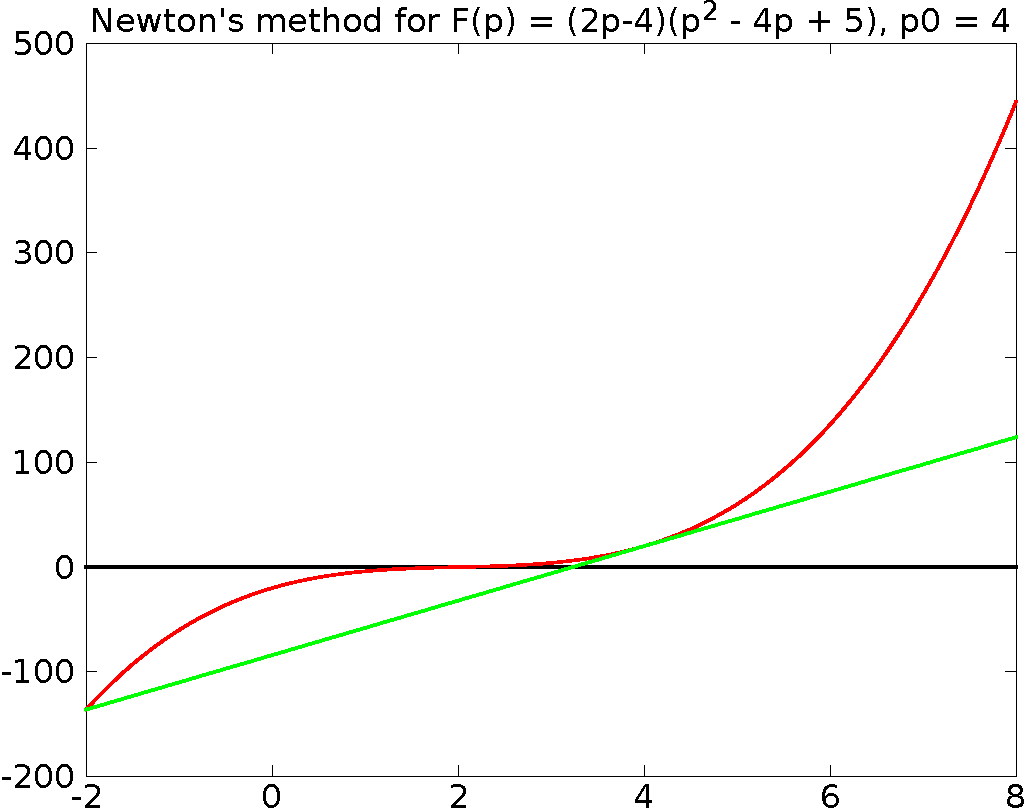
\includegraphics[width=2.8in]{fig1}}

\bigskip

Verify that $\delta p = -10/13 \approx -0.76923$.

\end{frame}


\begin{frame}
\frametitle{Iterative minimization}
\framesubtitle{Minimizing the linearized $\vec{f}$}

Problem with Newton's method: the Hessians
\begin{equation*}
\begin{bmatrix}
\frac{\partial^2 f_i}{\partial p_1^2} &
\frac{\partial^2 f_i}{\partial p_1 \partial p_2} & \cdots \\
\vdots & \vdots & \vdots \\
\frac{\partial^2 f_i}{\partial p_M \partial p_1} &
\frac{\partial^2 f_i}{\partial p_M \partial p_2} & \cdots
\end{bmatrix}
\end{equation*}
are tedious and expensive to calculate, especially if $M$, the
dimensionality of the parameter vector, is large.

\end{frame}


\begin{frame}
\frametitle{Iterative minimization}
\framesubtitle{Minimizing the linearized $\vec{f}$}

Because of the difficulty of calculating Hessians we typically use
quick-and-dirty approximations rather than explicitly calculate them.

\medskip

The \alert{Gauss-Newton} algorithm drops the second-order terms
entirely.

\medskip

The \alert{Levenberg-Marquardt} algorithm approximates the second
order terms by a scaled identity matrix:
\begin{equation*}
\left[ \mat{J}_{\vec{f}}^T(\vec{P})\mat{J}_{\vec{f}}(\vec{P}) +
\mu\mat{I} \right] \delta{\vec{P}} =
-\mat{J}^T_{\vec{f}}(\vec{P})\vec{f}(\vec{P}).
\end{equation*}
where the parameter $\mu$ is adapted during optimization.

\medskip

Lucky for us, Levenberg-Marquardt is implemented in many packages:
Matlab {\tt lsqnonlin()}, Octave {\tt leasqr()}, and {\em Numerical
Recipes in C} {\tt mrqmin()}.

\medskip

See the text, Appendix 6, for information on adapting
Levenberg-Marquardt to very large problems.

\end{frame}

\begin{frame}
\frametitle{Iterative minimization}
\framesubtitle{Iterative minimization applied to homography estimation}

In the case of \alert{homography estimation},
we have a set of 2D coordinates
of corresponding points $\vec{x}_i$ and $\vec{x}_i'$, so the
dimensionality of the \alert{measurement space} is $N=4n$ and the
measurement is a vector $\vec{X} \in \Rset^N$.

\medskip

Suppose our \alert{parameterization} was to choose a set of points
$\hat{\vec{x}}_i$ in the first image, then choose a homography
$\mat{H}$.
\begin{itemize}
\item The corresponding points
  $\hat{\vec{x}}_i'=\hat{\mat{H}}\hat{\vec{x}}_i$ would then be
  \alert{fixed}.
\item The \alert{parameter vector} $\vec{P} \in \Rset^M$, then, would
  contain the $2n$ parameters of $\hat{\vec{x}}_i$ and the 9
  parameters of $\hat{\mat{H}}$, so $M=2n+9$.
\item The resulting \alert{model} (the set of measurements in
  $\Rset^N$ that can be be generated with our parameterization) is a
  $2n+8$ dimensional submanifold $S \subset \Rset^N$.
\end{itemize}

\medskip

[Analogy: think about a circle as a 1D submanifold of $\Rset^2$.]

\end{frame}

\begin{frame}
\frametitle{Iterative minimization}
\framesubtitle{Iterative minimization applied to homography estimation}

Given the model in the previous page, it is straightforward to write
the mapping
\begin{equation*}
  \vec{f} : (\vec{h},\hat{\vec{x}}_1,\ldots,\hat{\vec{x}}_n) \mapsto
  (\hat{\vec{x}}_1,\hat{\vec{x}}_1',\ldots,\hat{\vec{x}}_n,\hat{\vec{x}}_n')
\end{equation*}
where $\hat{\vec{x}}_i' = \mat{H}\hat{\vec{x}}_i$.

\medskip

The reprojection error cost function becomes
$\|\vec{X}-\vec{f}(\vec{P})\|^2$, which is just the Mahalanobis cost
function with $\mat{\Sigma}=\mat{I}$.

\medskip

This means Levenberg-Marquardt applies.  The resulting algorithm is
Hartley and Zisserman's \alert{Gold Standard} MLE algorithm for
estimating $\mat{H}$.

\end{frame}

%--------------------------------------------------------------------
\section{Gold Standard algorithm}
%--------------------------------------------------------------------

\begin{frame}
\frametitle{Gold Standard algorithm}
\framesubtitle{The idea}

The \alert{Gold Standard algorithm} for $\mat{H}$ tries to find
\begin{equation*}
(\hat{\mat{H}},\hat{\vec{x}}_1,\ldots,\hat{\vec{x}}_n) =
\argmax_{\hat{\mat{H}},\hat{\vec{x}}_1,\ldots,\hat{\vec{x}}_n}
P(\vec{x}_1,\vec{x}_1',\ldots,\vec{x}_n,\vec{x}_n' \mid
\mat{H},\hat{\vec{x}}_1,\ldots,\hat{\vec{x}}_n)
\end{equation*}

\medskip

We know that maximizing the likelihood in the equation, assuming
Gaussian measurement error, means minimizing the reprojection error
\begin{equation*}
\sum_i d(\vec{x}_i, \hat{\vec{x}}_i)^2 +
       d(\vec{x}_i', \hat{\mat{H}}\hat{\vec{x}}_i)^2
\end{equation*}

\medskip

This is a nonlinear least squares problem, which Levenberg-Marquardt
can solve, but we need an \alert{initial solution}, which we can
obtain using the DLT.

\end{frame}

\begin{frame}
\frametitle{Gold Standard algorithm}
\framesubtitle{The algorithm}

\begin{block}{Gold Standard for $\mat{H}$: Objective}
  Given $n>4$ image point correspondences $\{\vec{x}_i \leftrightarrow
  \vec{x}_i' \}$, determine the maximum likelihood estimate
  $\hat{\mat{H}}$.
\end{block}

\begin{block}{Gold Standard }%for $\mat{H}$: Algorithm}
\begin{itemize}
\item[(i)] Compute an initial estimate of $\hat{\mat{H}}$ using
  the normalized DLT.
\item[(ii)] Compute an initial estimate of the subsidiary variables
  $\{\hat{\vec{x}}_i\}$ using $\{\vec{x}_i\}$ (see text for a better
  way).
\item[(iii)] Minimize the cost
\begin{equation*}
\sum_i d(\vec{x}_i, \hat{\vec{x}}_i)^2 +
       d(\vec{x}_i', \hat{\mat{H}}\hat{\vec{x}}_i)^2
\end{equation*}
  over $\hat{\mat{H}},\hat{\vec{x}}_1,\ldots,\hat{\vec{x}}_n$, using
  Levenberg-Marquardt over $2n+9$ variables: $2n$ for the points
  $\{\hat{\vec{x}}_i\}$ and 9 for the homography matrix
  $\hat{\mat{H}}$.
\end{itemize}
\end{block}

\end{frame}

\begin{frame}
\frametitle{Gold Standard algorithm}
\framesubtitle{Example code}

For example code for the Gold Standard
algorithm in Octave, see \texttt{gs\_demo.m} on
the course Web site.

\medskip

Note that if you're using Matlab you can use the Matlab port of the
Octave \texttt{leasqr()} function or use the Matlab Optimization Toolbox
function \texttt{lsqnonlin()}.  But be careful as the two functions work
a bit differently.

\end{frame}

%--------------------------------------------------------------------
\section{Robust estimation}
%--------------------------------------------------------------------

\begin{frame}
\frametitle{Robust estimation}
\framesubtitle{Introduction}

The Gold Standard algorithm is optimal if the \alert{measurement
  error} for the corresponding points $\vec{x}_i \leftrightarrow
\vec{x}_i'$ is actually \alert{Gaussian}.

\medskip

In practice, though, the points and their correspondences are obtained
through an \alert{automatic} procedure which makes \alert{mistakes}.

\medskip

These mistakes, or \alert{outliers}, will severely disrupt our
estimates, so they should be removed.

\medskip

We seek to obtain a set of \alert{inliers} that will be used for
estimation and a set of \alert{outliers} that will be ignored.

\medskip

This task is called \alert{robust estimation} because we want the
estimation method to be \alert{robust} to \alert{outliers} following
an unmodeled error distribution.

\end{frame}

\begin{frame}
\frametitle{Robust estimation}
\framesubtitle{RANSAC motivation}

Example: fitting a line $x'=ax+b$ to a set of points.

\medskip

\begin{columns}
\column{2.2in}
\myfig{2.1in}{HZ-fig3-7a}{Least squares fit is skewed by outliers.}
\column{2.2in}
\myfig{2.1in}{HZ-fig3-7b}{RANSAC support for two candidate lines.}
\end{columns}

\medskip

The \alert{RANSAC} (Random Sample Consensus, Fischler and Bolles,
1981) algorithm is one of the many robust methods to solve this
problem.

\end{frame}

\begin{frame}
\frametitle{Robust estimation}
\framesubtitle{RANSAC idea}

The idea of RANSAC is that we only need two points to determine a
line.

\medskip

So to begin, we pick two points \alert{at random} to define a line.

\medskip

The \alert{support} for this line is the number of points that lie
within a distance threshold $t$ of that line.

\medskip

We repeat for a while, and the \alert{line with the most support} is
deemed best.

\medskip

The points within the threshold are called \alert{inliers} and they
are said to make up the \alert{consensus set}.

\medskip

In the figure, we see that the line $\overline{\vec{a}\vec{b}}$ has a
support of 10 but the line $\overline{\vec{d}\vec{e}}$ has a support
of only 2.  We would select $\overline{\vec{a}\vec{b}}$ as a better
fit to the data than $\overline{\vec{d}\vec{e}}$.

\end{frame}

\begin{frame}
\frametitle{Robust estimation}
\framesubtitle{RANSAC algorithm}

Hartley and Zisserman's (2004) adaptation of Fischler and Bolles'
(1981) RANSAC:

\begin{block}{RANSAC: Objective}
Robust fit of a model to a data set $S$ which contains outliers
\end{block}

\begin{block}{RANSAC: Algorithm}
\begin{itemize}
\item[(i)] Randomly select a sample $s$ from $S$ and instantiate the
  model from $s$.
\item[(ii)] Find the consensus set (inliers) $S_i$ within distance
  threshold $t$ of the model.
\item[(iii)] If $|S_i|\ge T$ re-estimate the model using all of the
  points in $S_i$ and terminate; otherwise repeat from (i).
\item [(iv)] After $N$ trials, select the largest consensus set $S_i$
  and re-estimate the model using all of the points in $S_i$.
\end{itemize}
\end{block}

\end{frame}

\begin{frame}
\frametitle{Robust estimation}
\framesubtitle{RANSAC parameters}

RANSAC has three \alert{free parameters}:
\begin{itemize}
\item $t$: the \alert{distance threshold},
\item $T$: the \alert{minimum number of inliers} for early termination,
\item $N$: the \alert{number of samples}.
\end{itemize}

\medskip

$t$ can be determined empirically, or, if the \alert{error
  distribution} is \alert{known} to be Gaussian with standard
deviation $\sigma$, a 95\% or similar confidence interval can be
calculated.

\medskip

See Table 4.2 in the text for reasonable values of $t$ for various
vision problems.

\end{frame}

\begin{frame}
\frametitle{Robust estimation}
\framesubtitle{RANSAC parameters}

$N$ can be determined empirically, or if the proportion $w$ of inliers
is approximately known, we can choose $N$ giving (e.g.) a 99\%
probability that \alert{on some iteration} we will choose a sample
containing \alert{inliers only}.

\medskip

Example: in homography estimation our sample size would be 4.  If we
assume a 50\% outlier rate, we should select $N=72$ samples to assure
a 99\% probability of sampling at least one set with 4 inliers.

\medskip

See Table 4.3 in the text for some example values and how to calculate
$N$ in general.

\medskip

$T$, the acceptable consensus set size, should be approximately the
\alert{number of inliers} thought to be in the data.

\medskip

For example, in the case of homography estimation, if we have 100
correspondences and a 50\% outlier rate, we should let $T=50$.

\end{frame}

\begin{frame}
\frametitle{Robust estimation}
\framesubtitle{Adaptive version of RANSAC for unknown $w$}

One variant, when the percentage of inliers $w$ is unknown, is
\alert{adpative RANSAC}:
\begin{itemize}
\item Initialize $N=\infty$.
\item While running RANSAC, decrease $N$ whenever you obtain a sample
  with a bigger consensus set than previously seen.
\item Terminate after $N$ iterations.
\end{itemize}

\medskip

A bigger consensus set means $w$ is bigger
than previously thought, so $N$ need not be so large.

\end{frame}

\begin{frame}
\frametitle{Robust estimation}
\framesubtitle{Robust maximum likelihood estimation}

Note that step (iv) of RANSAC was to re-estimate the model from
\alert{all of the points} in $S_i$.  We should use maximum likelihood
in this case.

\medskip

\alert{Problem}: the set of inliers could \alert{change} after we
compute the new maximum likelihood model.

\medskip

We could just \alert{accept the estimate anyway}.

\medskip

Some approaches \alert{recompute the inliers} after obtaining the
maximum likelihood model then \alert{repeat} maximum likelihood model
estimation until the consensus set converges.

\medskip

See text for detailed discussion and other alternative approaches.

\end{frame}

\begin{frame}
\frametitle{Robust estimation}
\framesubtitle{Using RANSAC to estimate $\mat{H}$}

\begin{block}{Automatic $\mat{H}$ estimation: Objective}
  Given two images, compute the homography.
\end{block}

\begin{block}{Automatic $\mat{H}$ estimation: Algorithm}
\begin{itemize}
\item[(i)] Compute a set of \alert{interest points} in each image.
\item[(ii)] Compute \alert{putative correspondences} between the point
  sets.
\item[(iii)] \alert{RANSAC robust estimation}: Repeat for $N$ samples,
  where $N$ is determined adaptively as previously described:
  \begin{itemize}
  \item[(a)] Select a random sample of 4 correspondences and compute
    $\mat{H}$.
  \item[(b)] Calculate the distance $d_{\perp}$ for each putative
    correspondence.
  \item[(c)] Find the number of inliers for which $d_{\perp} < t =
    \sqrt{5.99}\sigma$ pixels.
  \end{itemize}
\item[(iv)] Re-estimate $\mat{H}$ using the inliers and the Gold
  Standard algorithm
\item[(v)] (Optional) use the new $\mat{H}$ to recompute the matching set of
  interest points and repeat from (iv) until convergence.
\end{itemize}
\end{block}

\end{frame}

\begin{frame}
\frametitle{Robust estimation}
\framesubtitle{Using RANSAC to estimate $\mat{H}$}

There are two implementation details that need consideration: how to
measure the distance and how to select the samples.
\begin{itemize}
\item For distance, the \alert{symmetric transfer error}
  $d^2_{\text{transfer}} = d(\vec{x},\mat{H}^{-1}\vec{x}')^2 +
  d(\vec{x}',\mat{H}\vec{x})^2$ is appropriate since it is easy to
  compute.  Reprojection error is better but expensive.
\item Widespread distribution of the samples is good, to ensure good
  interpolation in the rest of the image.  The sampler can be biased
  to pick points in different regions of the image rather than
  uniformly.
\end{itemize}

\end{frame}

\begin{frame}
\frametitle{Robust estimation}
\framesubtitle{Example results}

Example initial images (Hartley and Zisserman, 2004, Fig.\ 4.9):

\medskip

\begin{columns}[T]
\column{2.25in}
\myfig{2.2in}{HZ-fig3-9a}{Image 1}
\column{2.25in}
\myfig{2.2in}{HZ-fig3-9b}{\parbox{2in}{Image 2, related by rotation
    around camera center}}
\end{columns}

\end{frame}

\begin{frame}
\frametitle{Robust estimation}
\framesubtitle{Example results}

Detected corners, about 500 on each image.

\begin{columns}[T]
\column{2.25in}
\myfig{2.2in}{HZ-fig3-9c}{}
\column{2.25in}
\myfig{2.2in}{HZ-fig3-9d}{}
\end{columns}

\end{frame}

\begin{frame}
\frametitle{Robust estimation}
\framesubtitle{Example results}

Initial set of 268 correspondences obtained by SSD of image patches
around the corners:

\medskip

\begin{columns}[T]
  \column{2.25in} \myfig{2.2in}{HZ-fig3-9e}{\parbox{2in}{268 putative
      correspondences, Hartley and Zisserman (2004), Fig.\ 4.9(e)}}
  \column{2.25in} \myfig{2.2in}{HZ-fig3-9f}{\parbox{2in}{117/268
      outliers, Hartley and Zisserman (2004), Fig.\ 4.9(f)}}
\end{columns}

\end{frame}

\begin{frame}
\frametitle{Robust estimation}
\framesubtitle{Example results}

Final set of 262 correspondences after RANSAC, guided matching, and MLE.

\medskip

\begin{columns}[T]
  \column{2.25in} \myfig{2.2in}{HZ-fig3-9g}{\parbox{2in}{151 inliers
      consistent with $\mat{H}$ found by RANSAC, Hartley and Zisserman
      (2004), Fig.\ 4.9(g).}}  \column{2.25in}
  \myfig{2.2in}{HZ-fig3-9h}{\parbox{2in}{Final set of 262
      correspondences after guided matching and MLE beginning from the
      RANSAC solution, Hartley and Zisserman (2004), Fig.\ 4.9(h).}}
\end{columns}

\end{frame}

\begin{frame}
\frametitle{Robust estimation}
\framesubtitle{Implementation}

See the course Web site for a test using OpenCV, its built-in
\alert{Shi-Tomasi feature detector} and its built-in RANSAC $\mat{H}$
estimation function.

\medskip

See the Torr toolbox at {\small
  \url{http://cms.brookes.ac.uk/staff/PhilipTorr/Code/master_code.htm}}
for a Matlab implementation using the \alert{Harris corner detector}.

\medskip

When there is significant rotation and/or scale in the image plane,
the \alert{SIFT} (Scale Invariant Feature Transform) feature detector is much
better than Harris or Shi-Tomasi.

\medskip

There is a large literature on feature detectors enabling
correspondence estimation over multiple views.

\medskip

Transform invariance matching will be very important when we move to
multiple views of a general scene and estimate the fundamental matrix
$\mat{F}$ rather than a homography $\mat{H}$.

\end{frame}

\end{document}

